\documentclass[titlepage, twocolumn, a4paper, 12pt]{article}
\usepackage[swedish]{babel}
\usepackage[utf8]{inputenc}
\usepackage{verbatim}
\usepackage{fancyhdr}
\usepackage{graphicx}
\usepackage{parskip}
\usepackage{enumerate}

% SourceCode
\usepackage{listings}
\usepackage{color}

% Include pdf with multiple pages ex \includepdf[pages=-, nup=2x2]{filename.pdf}
\usepackage[final]{pdfpages}
% Place figures where they should be
\usepackage{float}

% SourceCode
\definecolor{keywordcolor}{rgb}{0.5,0,0.75}
\lstset{
  inputencoding=utf8,
  language=Java,
  extendedchars=true,
  basicstyle=\scriptsize\ttfamily,
  stringstyle=\color{blue},
  commentstyle=\color{red},
  numbers=left,
  firstnumber=auto,
  numberblanklines=true,
  stepnumber=1,
  showstringspaces=false,
  keywordstyle=\color{keywordcolor}
  % identifierstyle=\color{identifiercolor}
}

% Float for text
\floatstyle{ruled}
\newfloat{kod}{H}{lop}
\floatname{kod}{Kodsnutt}

% vars
\def\title{Genetisk animation; rörelsemönster i 2D mha neuralt nät och genetisk algoritm}
\def\preTitle{Projekt}
\def\kurs{Emergenta system, 5DV017}
\def\namn{Andreas Jakobsson}
\def\mail{dit06ajs@cs.umu.se}

\def\namnTva{Anton Johansson}
\def\mailTva{dit06ajn@cs.umu.se}

\def\namnTre{Erik Rönnberg}
\def\mailTre{dit06erg@cs.umu.se}

\def\namnFyra{Ludvig Widman}
\def\mailFyra{dit06lwn@cs.umu.se}

\def\namnFem{Ragnar Asplund}
\def\mailFem{dit04rad@cs.umu.se}

\def\pathtocode{$\sim$dit06ajn/edu/emergenta-system/projektet/src}

\def\handledareEtt{Jonny Pettersson, jonny@cs.umu.se}
\def\handledareTva{Anders Broberg, bopspe@cs.umu.se}

\def\inst{datavetenskap}
\def\dokumentTyp{Projektrapport}

\begin{document}
\begin{titlepage}
  \thispagestyle{empty}
  \begin{small}
    \begin{tabular}{@{}p{\textwidth}@{}}
      UMEÅ UNIVERSITET \hfill \today \\
      Institutionen för \inst \\
      \dokumentTyp \\
    \end{tabular}
  \end{small}
  \vspace{10mm}
  \begin{center}
    \LARGE{\preTitle} \\
    \huge{\textbf{\kurs}} \\
    \vspace{10mm}
    \LARGE{\title} \\
    \vspace{15mm}
    \begin{large}
      \namn, \mail \\
      \namnTva, \mailTva\\
      \namnTre, \mailTre\\
      \namnFyra, \mailFyra\\
      \namnFem, \mailFem\\
      \texttt{\pathtocode}
    \end{large}
    \vfill
    \large{\textbf{Handledare}}\\
    \mbox{\large{\handledareEtt}}
    \mbox{\large{\handledareTva}}
  \end{center}
\end{titlepage}

\newpage
\mbox{}
\vspace{70mm}
\begin{center}
% Dedication goes here
\end{center}
\thispagestyle{empty}
\newpage

\pagestyle{fancy}
\rhead{\today}
\lhead{\footnotesize{\mail, \mailTva\\\mailTre, \mailFyra, \mailFem}}
\chead{}
\lfoot{}
\cfoot{}
\rfoot{}

\begin{abstract}
% TODO: Sammanfattning/abstract

\end{abstract}

\cleardoublepage
\newpage
\tableofcontents
\cleardoublepage

\cfoot{\thepage}
\pagenumbering{arabic}

\section{Frågeställning}
Kan vi återskapa Sims Rapport? WWKSD? What whould Karl Sims do? Bigup!


Abstract Sammanfattning
Introduction Introduktion
    - Några tidigare studier
    - Frågeställning/Syfte
    - Vad vi har gjort
Creature Control Kontroll av varelser
  - Sensorer
  - Effektorer (diff på Sims)
  - Neuroner
  
Physical simulation
Behavior Selection
Results
Future Work
Conclusions
Acknowledgements
    - Sims Gud Karl



\section{Introduktion}
% Introduktion till ämnet, inklusive översikt av tidigare studier
% \cite{flake}

I detta projekt har vi undersökt möjligheten att utveckla rörelsemönster för en enkel varelse med hjälp av genetiska algoritmer. Varelsen har ett neuralt nät som ”hjärna” och har formen av en ledad ”mask”.

\subsection{Karl Sims}
Karl Sims utforskar i Evolving Virtual Creatures \cite{sims} både hur varelsers form och deras beteenden kan utvecklas med hjälp av genetiska algoritmer (GA). Varelserna har sensorer och effektorer som är kopplade till in- och utnoder i ett neuralt nät. 

I sina försök använder Sims en GA för att optimera både struktur och vikter i det neurala nätet. Det nät han använder har i varje nod en av många matematiska funktioner; exempelvis sinus, summa, produkt, max, osv. Sims lät sina försök köra mellan 50 och 100 generationer och optimerade mot olika typer av beteenden som ex gång, simmande och hoppande rörelser. 

\subsection{Hugo de Garis}
Hugo de Garis forskning i \textit{GENETIC PROGRAMMING Evolutionary Approaches to Multistrategy Learning} \cite{garis} inriktar sig i störst utsträckning mot utveckling av hårdvara med hjälp av genetiska algoritmer. Han beskriver metoder som shaping (att i olika steg ändra definitionen för fitness) och talar om "utvecklingsbara system" med de avseendet att vissa system inte går att ge önskvärt beteende med hjälp av genetiska algoritmer. Han nämner att de inte finns något sätt att definitivt avgöra vilka system som är utvecklingsbara med fasta kriterier.

Garis har utvecklat en simulerad ödla som han kallar LIZZY \cite{garis}. LIZZY känner sin omvärld med två antenner och tar därigenom emot karaktäristiska signaler från tre sorters kreatur i dess omgivning; Mate, Prey och Predator. Med hjälp av ett neuralt nät och en genetisk algoritm lär sig sedan LIZZY att söka upp Prey och Mate, där vidta passande åtgärder, och att fly undan Predators.

\subsection{Syfte}
% Frågeställning fylls i här typ
%Survival of the fit

\section{Metodbeskrivning, Vad vi har gjort}
% Metodbeskrivning. Ska beskrivas så utförligt att läsaren ska kunna
% reproducera ert arbete
% Systemet består av tre stora delar. Den genetiska algoritmen (GA), Hjärnan och Fysiksimuleringen.


\subsection{Kontroll av varelser}
\subsubsection{Sensorer}
% Bodies, getXposiotion() typ!!!!! <<<<<<< typ jag skrev typ
%VADÅ TYP

%for (int i = 0, length = inputs.length; i < length; i++) {
%            float b1 = bodyList.get(i).getPosition().getY();
%            float b2 = bodyList.get(i+1).getPosition().getY();
%            inputs[i] = b1-b2;
%}
        
%EXAKT!

\subsubsection{Effektorer}
% Joints

\subsubsection{Neuralt nät}
% Neuroner
Varelsens hjärna består av ett neuralt nät som styr dess beteende. Det neurala nätet är vagt implementerat enligt Hopfields modell för neurala nät, se kapitel 13 i boken textit{Neural networks: a systematic introduction}, \cite{raul}. Varje nod i det neurala nätet har bågar till och från alla andra noder. Varje båge har en vikt.

För att mata nätet med indata tas värden emot och körs genom en sigmoid funktion $1/\frac{1}{e^{-x}}$.

Vid varje simuleringssteg i hjärnan beräknas ett värde i varje nod. Värdet beräknas som en summa av värdet från varje båge gånger dess vikt. På denna summa appliceras sedan sigmoidfunktionen så värdet hamnar mellan -1 och 1. 

%tänkte mig lista klasser här så det blir en systemöversikt? 
%\begin{enumerate}[(a)]
%\item ...  ...
%\item hej
%\end{enumerate}

\subsection{Simulering}
Fysiksimuleringen använder biblioteket \textit{phys2d} \cite{phys2d} för själva fysiken. Detta bibliotek är skrivet av Kevin Glass och är en Java-portning av Erin Catto's plattform \textit{box2d} \cite{box2d}. Denna platform valdes på grund av att den bygger på Java och gruppen besitter kompetens inom språket. I simuleringen har ett markplan skapats och på detta en varelse. 

Varelsen består av en mask med 4 leder och 5 kroppsdelar. Varje led kan röra sig 180 grader. Varje kroppsdel har en sensor som ger \textit{hjärnan} indata om dess y-position i förhållande till delen utmed. Att en maskliknande varelse har valts beror på att kroppen är relativ enkel i sin sammansättning och komplexiteten sjunker således. Kroppsdelarnas vikt, ledernas typ och ledernas rörelsefrihet har valts efter eget tycke då varelsen ses som ett inledande exempel på hur systemet kan fungera. Valet av indata för varelsen grundas i en önskan om ledernas vetskap om varandra.


\subsection{Genetisk algoritm}
För selektion används en variant på tournament selection. Två grupper om tre individer väljs slumpmässigt och de med högst fitness ur respektive grupp korsas så två nya varelser med en blandning av deras genotyp skapas. Detta upprepas tills en bestämd del av en ny population har skapats. Därefter väljs fler grupper av tre där de bästa direkt går till den nya populationen oförändrade tills den nya populationen har samma storlek som den gamla. Varje individ i den nya populationen muterar varje del av sin genotyp med en viss sannolikhet. Den nya populationen ersätter därefter den gamla. 
		
Genotypen i varelsen kodar för vikter i det neurala nät som utgör dess hjärna. För att evaluera fitness för varje individ skapas ett nät med de vikter genotypen anger, detta får sedan under en begränsad tid styra en fast kropp i en fysiksimulering. Fitness beräknas på hur långt kroppen lyckats röra sig.

\section{Resultat}
% Resultat innehållande sammanställning/analys av tester
\begin{figure}
    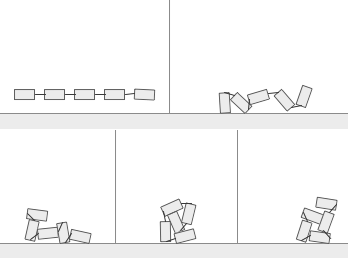
\includegraphics[width=78mm]{images/mask1_gs.png}
\end{figure}

\begin{figure}
    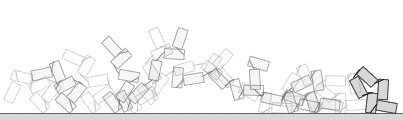
\includegraphics[width=78mm]{images/maskninja.png}
\end{figure}
\section{Diskussion}
% Diskussion av resultatet, koppling till tidigare studier

\bibliographystyle{alpha}
\bibliography{books}

\newpage
\appendix
\pagenumbering{roman}
\section{Källkod}\label{sec:kallkod}
Härefter följer utskrifter från källkoden och andra filer som hör till
denna laboration.

\subsection{Flocking.nlogo}\label{app:Flocking.nlogo}
\begin{footnotesize}
  \verbatiminput{../src/Flocking.nlogo}
\end{footnotesize}
\end{document}
